\documentclass{article}
\usepackage[margin=.9in]{geometry}
\usepackage[dvipsnames]{xcolor}
\usepackage{amsmath}
\usepackage{amssymb}
\usepackage{amsthm}
\usepackage{mathrsfs}
\usepackage{tikz}
\usepackage{csquotes}
\usepackage{float}
\newtheorem*{claim}{Claim}
\newtheorem*{poof}{Proof}
\title{HW 5}
\author{Christopher Hunt}
\date{}
\usepackage{graphicx} 
\usepackage{fancyhdr}

\begin{document}
\pagestyle{fancy}
\fancyhf{}
\rfoot{MTH 231}
\lfoot{Christopher Hunt}
\lhead{HW 5}
\rhead{\thepage}
\maketitle

\section*{16. Describe a set in terms of $A$ and $B$ (using set notation) which has the following Venn diagram:}
\begin{center}
  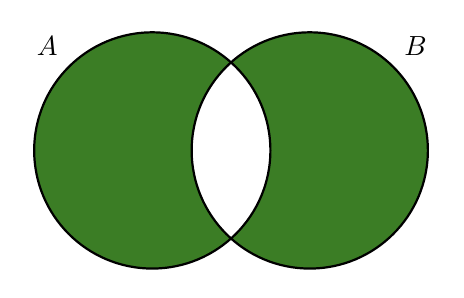
\begin{tikzpicture}[thick,
      set/.style = { circle, minimum size = 3cm}]
   
  % Set B
  \node[set,fill=OliveGreen,label={45:$B$}] (B) at (0:2) {};
   
  % Set A
  \node[set,fill=OliveGreen,label={135:$A$}] (A) at (0,0) {};
  \begin{scope}
      \clip (0,0) circle(1.5cm);
      \clip (2,0) circle(1.5cm);
      \fill[white](0,0) circle(1.5cm);
    
  \end{scope} 
  % Circles outline
  \draw (0,0) circle(1.5cm);
  \draw (2,0) circle(1.5cm);
     
  \end{tikzpicture}
\end{center}

\noindent This Venn Diagram can be written as \enquote{The union of the sets $A-B$ and $B-A$}. In set builder notation this will be:
$$ A-B \cup B-A$$

\noindent To demonstrate this consider these two sets:
\begin{align*}
    A&=\{1,2,3,4\}\\
    B&=\{3,4,5,6\}
\end{align*}
Now subtract $B$ from $A$ and $A$ from $B$:
\begin{align*}
    A-B&=\{1,2\}\\
    B-A&=\{5,6\}
\end{align*}
Now take the union of these two values:
\begin{align*}
    A-B\cup B-A&=\{1,2,5,6\}
\end{align*}
This produces the Venn diagram above.
\newpage

\section*{25. Let $A$, $B$, and $C$ be sets.}
\subsection*{a. Suppose that $A \subseteq B$ and $B \subseteq C$. Does this mean that $A \subseteq C$?}
\begin{claim}
    If $A \subseteq B$ and $B \subseteq C$, then $A \subseteq C$.
\end{claim}
\begin{poof}
    Assume $A \subseteq B$ and $B \subseteq C$ is true. By the definition of a subset we can state that every element $x$ in $A$ is an element in $B$ and every element $y$ in $B$ is an element of $C$. This can be visualually demosntrated using this Venn diagram:
    \begin{center}
        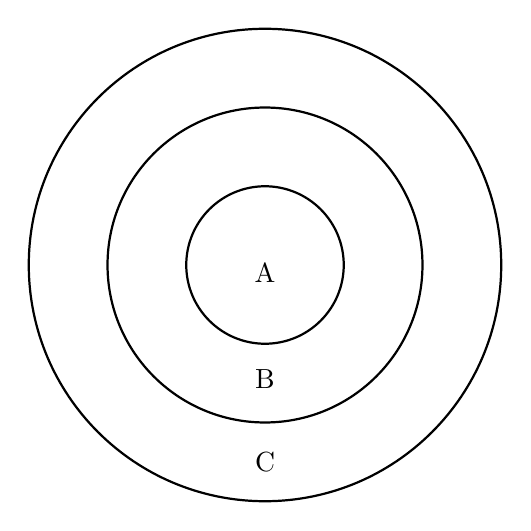
\begin{tikzpicture}[thick]
          % Draw outer circle (C)
          \draw (0,0) circle (3cm);
          \node[text=black] at (0,-2.5cm) {C};
          % Draw middle circle (B)
          \draw (0,0) circle (2cm);
          \node[text=black] at (0,-1.45cm) {B};
          % Draw inner circle (A)
          \draw (0,0) circle (1cm);
          \node[text=black] at (0,-.10cm) {A};
        \end{tikzpicture}
    \end{center}
    Since, every element of $B$ must be in $C$ and every element of $A$ must be in $B$ it follows that every element of $A$ must also be in $C$. Therefore, $A \subseteq C$ is true and the  from that the original claim is true. \\
    \qed
\end{poof}


\subsection*{b. Suppose that $A \in B$ and $B \in C$. Does this mean that $A \in C$? Give an example to prove that this does NOT always happen.}
\begin{claim}
    If $A \in B$ and $B \in C$, then $A \in C$.
\end{claim}
\begin{poof}
    For this claim to be false we must find a case where $A \in B$ and $B \in C$ is true but $A \in C$ is false. Consider the following sets, $A$, $B$, and $C$:
    \begin{align*}
        A &= \{1,2\}\\
        B&= \{A,3\}\\
        C&=\{B,4\}
    \end{align*}  
    These sets fullfil the antecedent of the claim above. They can also be expressed like:
    \begin{align*}
        A &= \{1,2\}\\
        B&= \{\{1,2\},3\}\\
        C&=\{\{\{1,2\},3\},4\}
    \end{align*}
    Viewing the expressions this way we can see that A is an element of an element of $C$ but not directly an element itself, which violates the claim that $A$ is an element of $C$ if $A$ is an element of $B$ and $B$ is an element of $C$. Therefore the claim is not always true.\\  
    \qed
\end{poof}

\newpage

\section*{SQ-4. For all sets $A$ and $B$,}
\subsection*{a. Prove that $A$ is a subset of $B$ if and only if $B^c$ is a subset of $A^c$.}
\begin{claim}
    $A \subseteq B \leftrightarrow B^c \subseteq A^c$
\end{claim}
\begin{poof}
    This bidirectional claim can be broken down into two implications:
    \begin{align*}
        1.&\;A\subseteq B \rightarrow B^c\subseteq A^c\\
        2.&\;B^c\subseteq A^c \rightarrow A\subseteq B
    \end{align*}
    Let's assume the antecedant of claim one to be true. That is $A$ is a subset of $B$.
    \begin{figure}[H]
    \centering
        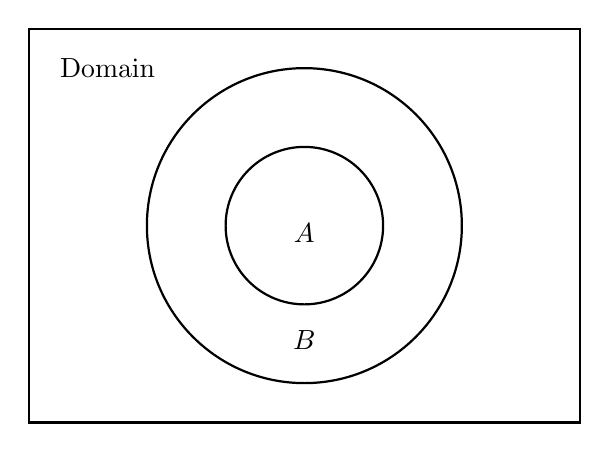
\begin{tikzpicture}[thick]
          % Draw box
          \draw (-3.5cm,-2.5cm) rectangle (3.5cm,2.5cm);
          \node[text=black] at (-2.5cm, 2) {Domain};
          % Draw middle circle (B)
          \draw (0,0) circle (2cm);
          \node[text=black] at (0,-1.45cm) {$B$};
          % Draw inner circle (A)
          \draw (0,0) circle (1cm);
          \node[text=black] at (0,-.10cm) {$A$};
        \end{tikzpicture}
    \end{figure}
    Now consider $B^c$ and $A^c$ which are the areas in the domain which are outside the corresponding sets of $A$ and $B$. Since every element of $A$ is in $B$ we know that $A$ has less than or equal to the same number of elements as $B$. Taking their compliment we know that $B^c$ is less than or equal to $A^c$ and since all the elements in $A$ are also in $B$, we know that any element which is not in $B$ must also not be in $A$ which meets the definition of a subset. Therefore the implication is true.

    Now Let's assume the antecedent of the second claim is true. That is every element not in $B$ is also not in $A$.
    \begin{figure}[H]
        \centering
            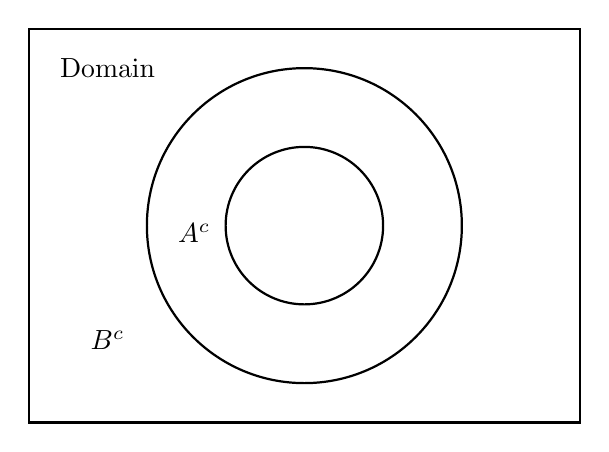
\begin{tikzpicture}[thick]
              % Draw box
              \draw (-3.5cm,-2.5cm) rectangle (3.5cm,2.5cm);
              \node[text=black] at (-2.5cm, 2) {Domain};
              % Draw middle circle (B)
              \draw (0,0) circle (2cm);
              \node[text=black] at (-2.5cm,-1.45cm) {$B^c$};
              % Draw inner circle (A)
              \draw (0,0) circle (1cm);
              \node[text=black] at (-1.4cm,-.10cm) {$A^c$};
            \end{tikzpicture}
        \end{figure}
    Due to this fact every element not in $A^c$ must also not be in $B^c$, that is every element in $A$ is also in $B$. Therefore the second claim holds. Since both claims are true then the original claim is also true. \\ 
    \qed

\end{poof}


\subsection*{b. Prove that if $A$ is a subset of $B$ and $B$ is a subset of $A$, then $A=B$.}
\begin{claim}
    $A \subseteq B \wedge B \subseteq A \rightarrow A = B$
\end{claim}
\begin{poof}
    Assume that $A \subseteq B$ and $B \subseteq A$ are both true. That is, every element of $A$ is an element of $B$ and every element of $B$ is an element of $A$. Consider some arbitrary element $x$ in the set $A$, this element will be in set $B$. Now, consider some other arbitrary element $y$ in set $B$, this element will be in set $A$ as well. Since there are no elements that can be found in $A$ that are not in $B$ and no elements that can be found in $B$ that are not in $A$, therefore $A$ and $B$ contain exactly the same elements. Therefore the claim is true. \\ 
    \qed
\end{poof}

\newpage

\section*{SQ-5. Prove or disprove: if $A$ is a subset of $B$, the $\mathscr{P}(A)$ is a subset of $\mathscr{P}(B)$.}
\begin{claim}
    $A \subseteq B \rightarrow \mathscr{P}(A) \subseteq \mathscr{P}(B)$
\end{claim}
\begin{poof}
    Assume $A \subseteq B$, that is, every element of $A$ is an element of $B$. Now consider an arbitrary element $x \in \mathscr{P}(A)$. Since $x$ is in the powerset of $A$ we know that $x \subseteq A$ and due to the transitive property of subsets (proof 25a) $x$ must be a subset of $B$ as well. Because $x \subseteq B$ it follows that $x \in \mathscr{P}(B)$. Since $x$ can be any arbitrary element of $\mathscr{P}(A)$, then it follows that $\mathscr{P}(A) \subseteq \mathscr{P}(B)$. Therefore, the claim is true.\\
    \qed

\end{poof}



\end{document}
